\documentclass{iopjournal}
\usepackage[round,authoryear]{natbib}
\setcitestyle{aysep={},notesep={, },citesep={,}}
\usepackage{url}
\usepackage{amsmath,amssymb,amsfonts}
\usepackage{gensymb}
\usepackage{algorithmic}
\usepackage{graphicx}
\usepackage{transparent}
\usepackage{siunitx}
\usepackage{textcomp}
\usepackage{xcolor, soul}
\usepackage{subcaption}
\usepackage{comment}
\usepackage{anyfontsize}
\usepackage[acronym,nonumberlist]{glossaries}
\usepackage{booktabs}
\usepackage{multirow}
\usepackage{array}
\usepackage{colortbl}
\usepackage{rotating}
\usepackage{makecell}
\usepackage{pifont}% for checkmarks
\usepackage{adjustbox}
\usepackage{changepage}
\usepackage{lipsum}% for lorem ipsum
\makeglossaries
\graphicspath{{figures/}}

% Override ragged right from class file to make text justified
\usepackage{ragged2e}
\justifying
\raggedbottom

% Citations blue, acronyms/internal links black
\hypersetup{
    colorlinks=true,
    linkcolor=black,
    citecolor=blue,
    urlcolor=blue
}
\def\BibTeX{{\rm B\kern-.05em{\sc i\kern-.025em b}\kern-.08em
    T\kern-.1667em\lower.7ex\hbox{E}\kern-.125emX}}

\newacronym{RF}{RF}{Radio Frequency}
\newacronym{EMF}{EMF}{Electromagnetic Field}
\newacronym{SAR}{SAR}{Specific Absorption Rate}
\newacronym{APD}{APD}{Absorbed Power Density}
\newacronym{BS}{BS}{Base Station}
\newacronym{UE}{UE}{User Equipment}
\newacronym{MISO}{MISO}{Multiple-Input Single-Output}
\newacronym{FDTD}{FDTD}{Finite-Difference Time-Domain}
\newacronym{TF/SF}{TF/SF}{Total-Field/Scattered-Field}
\newacronym{PW}{PW}{Plane Wave}
\newacronym{SNR}{SNR}{Signal-to-Noise Ratio}
\newacronym{MRT}{MRT}{Maximum Ratio Transmission}
\newacronym{IDM}{IDM}{Integrated Dose Model}
\newacronym{CPW}{CPW}{Cells Per Wavelength}
\newacronym{PML}{PML}{Perfectly Matched Layer}
\newacronym{CSF}{CSF}{Cerebrospinal Fluid}
\newacronym{ICNIRP}{ICNIRP}{International Commission on Non-Ionizing Radiation Protection}
\newacronym{MaMIMO}{MaMIMO}{Massive MIMO}
\newacronym{CFL}{CFL}{Courant-Friedrichs-Lewy}
\newacronym{UPML}{UPML}{Uniaxial Perfectly Matched Layer}
\newacronym{ViP}{ViP}{Virtual Population}
\newacronym{HPC}{HPC}{High-Performance Computing}
\newacronym{TDMA}{TDMA}{Time Division Multiple Access}

\newcommand{\headeretal}{et al.}
\newcommand{\cmark}{\ding{51}}% checkmark
\newcommand{\xmark}{\ding{55}}% x mark

% Define colors
\definecolor{lightgray}{gray}{0.92}
\definecolor{fr1color}{RGB}{230,242,255}
\definecolor{fr3color}{RGB}{255,242,230}
\definecolor{fr2color}{RGB}{242,255,230}

% Suppress the default articletype (journal name, dates, margin notes)
\renewcommand{\articletype}[1]{}

\usepackage[modulo]{lineno}% reviewer line numbers

\begin{document}
\linenumbers

\title{Supplementary Information for: Environmental and Auto-Induced RF-EMF Adult and Children Far-Field Exposure Simulations between 450 MHz and 26 GHz}
\author{Robin Wydaeghe$^{1,*}$\,\orcid{0000-0002-1374-0118}, Bram Stroobandt$^1$\,\orcid{0000-0003-2377-4300}, Silvia Gallucci$^2$\,\orcid{0009-0000-0481-1554}, Marta Parazzini$^2$\,\orcid{0000-0001-9008-7530}, Gabriella Tognola$^2$\,\orcid{0000-0002-2433-449X}, Joe Wiart$^3$\,\orcid{0000-0002-8902-5778}, Günter Vermeeren$^1$\,\orcid{0000-0002-5309-3808}, Mònica Guxens$^4$\,\orcid{0000-0002-8624-0333}, Emmeric Tanghe$^1$\,\orcid{0000-0003-0020-6466}, and Wout Joseph$^{1}$\,\orcid{0000-0002-8807-0673}}

\affil{$^1$Department of Information Technology, Ghent University - imec, WAVES Research Group, Technologiepark-Zwijnaarde 126, 9052 Ghent, Belgium}

\affil{$^2$Institute of Electronics, Computer and Telecommunication Engineering, National Research Council of Italy (CNR-IEIIT), Piazza Leonardo da Vinci 32, 20133 Milan, Italy}

\affil{$^3$Department of Communication and Electronic (COMELEC), Télécom Paris, Institut Polytechnique de Paris, 19 Place Marguerite Perey, 91120 Palaiseau, France}

\affil{$^4$ISGlobal, Barcelona Institute for Global Health, C/ Doctor Aiguader 88, 08003 Barcelona, Spain}

\affil{$^*$Author to whom any correspondence should be addressed.}

\email{robin.wydaeghe@ugent.be}


\section{Computational Methodology Details}

This supplementary document provides detailed technical information on the computational methodology used in the main study, including spatial and temporal discretization strategies, grid resolution trade-offs, and the rationale for frequency-dependent meshing decisions.

\subsection{Spatial and temporal discretization}
\label{si:discretization}

Spatial discretization followed a frequency-dependent scheme trading numerical accuracy against computational cost.
We targeted 10 \gls{CPW} in the highest-permittivity tissue at each frequency, keeping phase error below 1\% per wavelength~\citep{taflove2005computational}.
Figure~\ref{fig:gridding_justification} shows the grid trade-offs: panel (a) shows skin mesh perforation, (b) shows computational cost scaling, (c) shows cells spanning the 10~g averaging cube, and (d) shows cells per $\delta_{90}$.
Vitreous humor (the gel-like substance filling the eyeball) typically has the highest permittivity ($\varepsilon_r \approx 69$ at 450~MHz, $\approx 31$ at 26~GHz), making it the limiting tissue for grid resolution.

\begin{figure}
    \centering
    
\includegraphics[width=3.5in]{figures/gridding_justification_combined.pdf}
    \caption{Grid resolution trade-offs. (a)~Skin mesh perforation increases sharply above 2.5~mm cell size. (b)~Computational cost scales with the fourth power of cell size without height factor, or linearly with height factor below 0.6~mm. (c)~Cells spanning the 10~g \gls{SAR} averaging cube. (d)~Cells per $\delta_{90}$ for skin at 450~MHz, 7~GHz, and 26~GHz. Green, orange, and red regions indicate acceptable, transitional, and unacceptable ranges.}
    \label{fig:gridding_justification}
\end{figure}

At lower frequencies (450--1450~MHz), a uniform cell size of 2.5~mm was employed, yielding 32~\gls{CPW} in vitreous humor at 450~MHz and 10~\gls{CPW} at 1450~MHz.
In the FR1 band, the large Cartesian product of configurations (4 phantoms $\times$ 9 frequencies $\times$ 12 directions/polarizations = 432 simulations for environmental exposure) necessitated keeping the grid coarse where possible.
For intermediate frequencies (2140--5800~MHz), the step size was reduced to 1.0--1.7~mm, keeping \gls{CPW} values between 6 and 14 depending on tissue type (Table~I of main paper).
At 5.8~GHz, we retained a 1.0~mm step (rather than the 0.86~mm that would yield exactly 10~\gls{CPW}) to limit the computational cost of the many FR1 simulations.
At frequencies above 7~GHz, where fewer phantom-direction combinations were simulated, finer grids of 0.4--0.6~mm were used.
At 26~GHz, a 0.3~mm cell size provides 7~\gls{CPW} in vitreous humor, below the 10~\gls{CPW} target.
This is acceptable because the uncertainty in measured tissue dielectric properties (typically 10--20\% across studies~\citep{gabriel1996dielectric,kos2011exposure}) exceeds the numerical error from 7~\gls{CPW} discretization, and at 26~GHz the relevant metric (APD) is a surface quantity that does not require resolving the field distribution deep within the eye.

The time step was set to the maximum value allowed by the \gls{CFL} stability condition for 3D \gls{FDTD}~\citep{taflove2005computational}, $\Delta t = \Delta x_\mathrm{min} / (c_0 \sqrt{3})$, where $\Delta x_\mathrm{min}$ is the smallest grid step in any dimension.
The resulting time steps range from 4.81~ps at 450~MHz to 0.58~ps at 26~GHz (Table~I of main paper).
Operating at the CFL limit balances spatial and temporal discretization errors, minimizing phase error.

\subsection{Grid resolution trade-offs}

Electromagnetic penetration depth decreases with frequency, changing the dosimetric problem and grid resolution requirements.
Table~I in the main paper reports the 90\% power absorption depth ($\delta_{90}$) for skin, muscle, and vitreous humor, defined as the depth at which 90\% of incident power has been absorbed.
For a plane wave in a lossy dielectric, the electric field decays as $E(z) = E_0 e^{-\alpha z}$, where $\alpha$ is the attenuation constant.
Since power density scales as $|E|^2$, the 90\% absorption depth is
\begin{equation}
\delta_{90} = \frac{\ln(10)}{2\alpha} \,,
\end{equation}
where the attenuation constant $\alpha = -\mathrm{Im}(k)$ is derived from the complex propagation constant
\begin{equation}
k = \omega\sqrt{\mu_0 \varepsilon_0 \varepsilon_r^*} \,,
\end{equation}
with $\varepsilon_r^* = \varepsilon_r - j\sigma/(\omega\varepsilon_0)$ being the complex relative permittivity.

At 450~MHz, $\delta_{90}$ in skin is 61~mm, outside the 0.5--4~mm anatomical skin thickness.
At sub-GHz frequencies, energy penetrates deep into underlying tissues (fat, muscle, organs), and the \gls{SAR} distribution depends on the full three-dimensional anatomy.
At 26~GHz, $\delta_{90}$ drops to 1.1~mm, confining virtually all absorption to the skin and subcutaneous fat.

Figure~\ref{fig:gridding_justification}d shows how many cells span the 90\% absorption depth.
The ``Cells per $\delta_{90}$'' row in Table~I of the main paper indicates how many grid cells span the 90\% absorption depth.
Values range from 24 cells at 450~MHz to 4 cells at 26~GHz.
Fewer cells per $\delta_{90}$ is acceptable because the relevant metric at high frequencies (APD) is a surface integral that does not require resolving the exponential decay profile in detail.

Figure~\ref{fig:gridding_justification}a shows skin mesh perforation at coarse resolutions.
Skin mesh perforation also matters: at coarse resolutions, the voxelized skin develops holes where the mesh fails to capture thin anatomy.
The ``Perforation'' row in Table~I of the main paper quantifies this as the percentage of skin surface not covered by skin voxels after discretization.
We measured perforation by voxelizing each phantom at each frequency's resolution, then counting skin voxels visible from six cardinal directions.
At 2.5~mm resolution (450--1450~MHz), perforation is 13.1\%, meaning approximately one-eighth of the skin surface is represented by underlying tissue (fat or muscle).
This occurs primarily where skin is thinnest (eyelids, inner arms) or curvature is high (ears, fingers).
At 1.7~mm (2140~MHz), perforation drops to 1.0\%. At 1.5~mm and finer (2450~MHz+), the mesh closes completely.
Perforation minimally affects \gls{SAR} accuracy because at low frequencies where it occurs, penetration depth exceeds skin thickness: at 450~MHz, $\delta_{90} = 61$~mm while anatomical skin is only 0.5--4~mm.
Deeper tissues dominate the absorption pattern.
The 10~g averaging volume for psSAR$_{10\mathrm{g}}$ spans at least 21.5~mm per side, much larger than perforation holes, smoothing discretization artifacts.

\subsection{Age dependence of tissue dielectric properties}
\label{si:age}

The dielectric properties in this study come from the IT'IS database~\citep{itis_database}, which assigns one $(\varepsilon_r,\sigma)$ spectrum per tissue regardless of age.
The four phantoms therefore reproduce age-dependent anatomy but share adult tissue properties.
Age-independent properties are standard in numerical RF dosimetry~\citep{bakker2010children,kuehn2009assessment,gosselin2014development,hirata2021review}.
Here we quantify the error they introduce.
The penetration depth sets how deep this mismatch matters.
Above~3~GHz the skin $\delta_{90}$ is below~18~mm (Table~I in the main paper), so absorption concentrates in the skin and the surface metrics follow the normal-incidence Fresnel transmission
\begin{equation}\label{eq:T0}
T_0 = \frac{4\,\mathrm{Re}(\tilde{n})}{|1+\tilde{n}|^2} \,, \qquad \tilde{n} = \sqrt{\varepsilon_r^*} \,,
\end{equation}
where $\tilde{n}$ is the complex refractive index and $\varepsilon_r^*$ the complex relative permittivity defined above.
The age sensitivity of the \gls{APD} then reduces to that of $T_0$.

Younger tissue holds more water. This raises both $\varepsilon_r$ and $\sigma$ in the microwave band~\citep{peyman2009dielectric}.
\citet{peyman2009dielectric} measured child and adult skin from~450 to~2450~MHz. The child values were higher by~24\% in $\varepsilon_r$ and by~23--38\% in $\sigma$.
We apply this child-to-adult ratio to the adult skin used here, holding it frequency-independent above~2.45~GHz in line with the water-content mechanism.
The resulting $T_0$ then falls by~9.5\% at~450~MHz and by~6.9\% at~26~GHz, computed analytically from~\eqref{eq:T0} without additional simulation.
The wetter child skin reflects slightly more, so the adult-parameter simulation overestimates child surface absorption rather than underestimating it.
The tabulated parameters are themselves uncertain by~10--20\%~\citep{gabriel1996dielectric,kos2011exposure}.
Through~\eqref{eq:T0} this uncertainty propagates to only a~4--9\% band on $T_0$.
Figure~\ref{fig:age_sensitivity} compares the age shift with this band, and Table~\ref{table:age_sensitivity} lists it at four frequencies.
The two are of the same order. Age dependence is therefore no larger than the existing dielectric uncertainty.

Below~3~GHz the field reaches fat and muscle, where $\delta_{90}$ exceeds~20~mm.
Muscle is the dominant deep absorber. It stays water-rich at every age, so its dielectric properties barely change~\citep{gabriel2005age}.
A layered skin--fat--muscle model therefore gives the same skin-driven shift.
Averaging over incidence angle and polarisation reduces the effect further.
The flux-weighted, polarisation-averaged transmission changes by~6--8\%, less than the~7--10\% at normal incidence.
The transverse-magnetic age gap also shrinks toward zero as the angle approaches the pseudo-Brewster angle, near~$80^\circ$.
Normal incidence therefore bounds the angle-averaged effect.
Peak surface \gls{SAR} moves in the opposite direction by~2--11\%, the balancing effect reported by~\citet{gabriel2005age}.
\citet{peyman2009dielectric} measured below~10\% on psSAR$_{10\mathrm{g}}$. \citet{christ2010age} attribute child--adult differences to anatomy rather than dielectric properties, and report no systematic age dependence in head-averaged peak spatial SAR.
Compliance conclusions therefore do not change.

\begin{table}[tbp]
\centering
\caption{Effect of age-dependent skin dielectric properties on far-field metrics, child relative to the adult-parameter simulation, computed analytically from~\eqref{eq:T0}. $T_0$: normal-incidence transmission. $\bar{T}$: flux-weighted, polarisation-averaged transmission. $\delta_{90}$: 90\% power-absorption depth. All effects are of the same order as the~4--9\% that a~10--20\% dielectric-parameter uncertainty propagates onto $T_0$.}
\label{table:age_sensitivity}
\begin{tabular}{@{}lccc@{}}
\toprule
\textbf{Frequency} & \textbf{$\Delta T_0$ (APD)} & \textbf{$\Delta \bar{T}$} & \textbf{$\Delta \delta_{90}$} \\
 & \textbf{(\%)} & \textbf{(\%)} & \textbf{(\%)} \\
\midrule
450~MHz  & $-9.5$ & $-8.3$ & $-18.6$ \\
2450~MHz & $-7.6$ & $-6.5$ & $-9.2$ \\
5800~MHz & $-7.5$ & $-6.5$ & $-9.2$ \\
26~GHz   & $-6.9$ & $-5.9$ & $-9.3$ \\
\bottomrule
\end{tabular}
\end{table}

\begin{figure}[tbp]
    \centering
    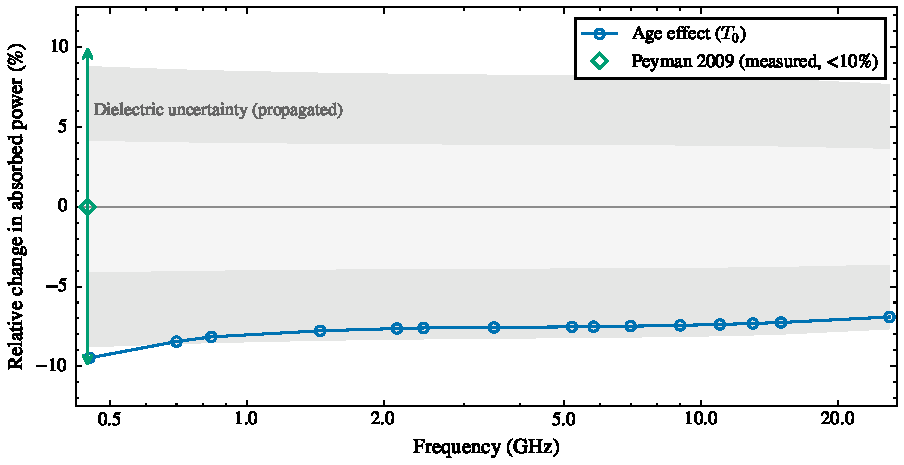
\includegraphics[width=\textwidth]{figures/r24_age_sensitivity.pdf}
    \caption{Age effect on absorbed power, child relative to the adult-parameter simulation (blue), from the closed-form Fresnel model. $T_0$ sets the \gls{APD} above~6~GHz and the whole-body \gls{SAR} below it, so the same relative change applies to both. The shaded band is the 10--20\% dielectric-parameter uncertainty propagated onto $T_0$, which gives~4--9\%. The measured child/adult skin sensitivity of~\citet{peyman2009dielectric} (green, $<$10\%) brackets it.}
    \label{fig:age_sensitivity}
\end{figure}

\subsection{Domain-truncation validation}
\label{si:truncation}

Two domain reductions keep the high-frequency simulations tractable: half-body symmetry and a height factor~$h$.
Both work because the penetration depth above~7~GHz is millimetric (Table~I in the main paper).
Absorption then concentrates near the illuminated surface, and the removed tissue carries negligible field.
Here we quantify the error in the dosimetric metrics through a convergence analysis against the retained domain size.

We compared full-body and truncated simulations at fixed phantom, frequency, incidence direction, and polarisation, varying only the retained height fraction~$h$.
The reference is the full body ($h=1$).
The sweep used $\theta$-polarised broadside incidence, the configuration that drives the strongest whole-body currents and so bounds the truncation error from above.
The sweep covered~450~MHz for Duke (adult) and Thelonious (child), and~3.5~GHz for Duke.
The truncation levels $h \in \{0.58, 0.42, 0.30\}$ match the FR3 values in Table~I of the main paper, applied here at the lowest frequency to maximise the truncation error.
Table~\ref{table:truncation} lists the deviation for every metric.

At~450~MHz the body spans about~2.6~wavelengths for the adult and~1.7 for the child.
The $\theta$-polarisation then drives a resonant longitudinal current along the whole body.
Truncating the body cuts this current.
The local and whole-body \gls{SAR} then move by up to~53\%.
The deviation grows with truncation severity.
It is non-monotonic, because each retained length samples a different point of the standing-wave pattern.
Truncation is therefore inadmissible near whole-body resonance.
For this reason the campaign keeps the full body ($h=1$) at all frequencies $\le 7$~GHz, where the full mesh also stays computationally tractable.

At~3.5~GHz the penetration depth is millimetric and absorption stays local to the illuminated upper body.
The same truncation ($h=0.30$, lower~70\% of the body removed) then leaves the local peak metrics unchanged.
The psSAR$_{10\mathrm{g}}$ shifts by~$-1.7\%$, the brain peak by~$+0.1\%$, and the eye peak by~$+0.01\%$.
Only mass-averaged quantities shift.
Whole-body \gls{SAR} is one such quantity.
Truncation removes absorbing tissue together with the mass over which the average is taken.
At broadside incidence the removed lower body still absorbs about~45\% of the total power at~7~GHz, so the truncated whole-body \gls{SAR} is not recovered by renormalising to the full-body mass.
The campaign therefore computes whole-body \gls{SAR} on the full body throughout, never on a truncated domain.

Height reduction is applied only above~7~GHz.
There the penetration depth is shorter than at~3.5~GHz, so the reported local metrics stay within the same~$<4\%$ bound.
The validation used plane-wave incidence, which illuminates the whole body uniformly.

The half-body symmetry reduction places a \gls{PML} boundary at the sagittal midplane.
Tissues that overlap with this plane may show non-physical \gls{SAR} rise with frequency. Their value is also much lower than exterior tissues at these higher frequencies.
The main-text analysis excludes the affected metrics on this basis, namely brain and genitals \gls{SAR} (Figure~8 in the main paper).
Tissues on the illuminated side lie many penetration depths from the cut, so their metrics are unaffected.

\begin{table}[tbp]
\centering
\caption{Domain-truncation error in the far-field \gls{SAR} metrics for a retained height fraction~$h$ relative to the full body ($h=1$), under $\theta$-polarised broadside incidence. Positive values overestimate. The 450~MHz and 3.5~GHz columns are controls. Height reduction is applied only above~7~GHz, where the reported metrics change by~$\le 4\%$. The large, non-monotonic 450~MHz errors reflect whole-body resonance and are discussed in the text.}
\label{table:truncation}
\begin{tabular}{@{}l rrr r r@{}}
\toprule
 & \multicolumn{3}{c}{450~MHz (\%)} & 3.5~GHz (\%) & 7~GHz (\%) \\
\cmidrule(lr){2-4} \cmidrule(lr){5-5} \cmidrule(lr){6-6}
\textbf{Metric} & $h{=}0.30$ & $h{=}0.42$ & $h{=}0.58$ & $h{=}0.30$ & $h{=}0.30$ \\
\midrule
\multicolumn{6}{@{}l}{\textit{Duke (adult)}} \\
\multicolumn{6}{@{}l}{\textit{Peak spatial-average SAR (10\,g)}} \\
\quad whole body & $+12.8$ & $+6.5$ & $-5.5$ & $-1.7$ & $+0.6$ \\
\quad brain & $+13.7$ & $+0.1$ & $+7.9$ & $+0.1$ & $+0.1$ \\
\quad eyes & $+9.4$ & $-7.6$ & $+4.2$ & $+0.0$ & $-0.1$ \\
\quad skin & $+17.9$ & $+11.2$ & $-3.7$ & $-1.7$ & $+0.8$ \\
\multicolumn{6}{@{}l}{\textit{Mass-averaged SAR}} \\
\quad whole body & $+20.4$ & $+0.2$ & $-12.2$ & $+6.2$ & $+3.1$ \\
\quad brain & $+8.8$ & $-5.8$ & $+7.7$ & $+1.2$ & $+1.2$ \\
\quad eyes & $+18.7$ & $-5.1$ & $+13.6$ & $+1.2$ & $+1.2$ \\
\quad skin & $+24.0$ & $+2.2$ & $-6.8$ & $+8.7$ & $+2.5$ \\
\midrule
\multicolumn{6}{@{}l}{\textit{Thelonious (child)}} \\
\multicolumn{6}{@{}l}{\textit{Peak spatial-average SAR (10\,g)}} \\
\quad whole body & $-52.8$ & $-42.6$ & $-5.8$ & $-3.5$ & $+0.1$ \\
\quad brain & $-27.0$ & $-4.7$ & $-8.0$ & $+0.1$ & $-0.7$ \\
\quad eyes & $-22.2$ & $+2.3$ & $-7.3$ & $-1.9$ & $-1.4$ \\
\quad skin & $-50.4$ & $-39.7$ & $-5.3$ & $-3.5$ & $+0.1$ \\
\multicolumn{6}{@{}l}{\textit{Mass-averaged SAR}} \\
\quad whole body & $-29.4$ & $-19.6$ & $-15.5$ & $+3.2$ & $+2.5$ \\
\quad brain & $-26.4$ & $-9.8$ & $-8.2$ & $+0.5$ & $-0.9$ \\
\quad eyes & $-36.5$ & $-14.4$ & $-15.6$ & $-2.7$ & $+0.8$ \\
\quad skin & $-9.6$ & $-6.2$ & $-2.5$ & $+3.8$ & $+2.7$ \\
\bottomrule
\end{tabular}
\end{table}

\subsection{Uncertainty budget}
\label{si:uncertainty}

The reported \gls{SAR} and \gls{APD} carry uncertainty from the model inputs and from the numerical method.
We follow the GUM framework~\citep{jcgm2008uncertainty} and the uncertainty guidance of IEC/IEEE~62704-1~\citep{iec62704}.
Each input has a standard uncertainty, one standard deviation.
We combine the independent random contributions in quadrature.
A coverage factor of~2 then scales the result to about a 95\% coverage probability, the expanded uncertainty.
Two effects act in one direction, so we list them separately.
Table~\ref{table:uncertainty} lists the budget. Figure~\ref{fig:uncertainty} ranks the contributions.

The tabulated dielectric parameters carry a~10--20\% spread~\citep{gabriel1996dielectric,kos2011exposure}.
Through the Fresnel transmission this propagates to a~4--9\% band on the absorbed power (Section~\ref{si:age}).
We take~$\pm 9\%$ as the bound. A uniform distribution then gives a standard deviation of~$9\%/\sqrt{3} = 5.2\%$.
This is the dominant term.

The \gls{FDTD} scheme contributes spatial and temporal error.
Spatially, the grid holds at least~10~\gls{CPW} in bulk tissue, where the Yee dispersion error is~1\% per wavelength (Section~\ref{si:discretization}).
The vitreous humor of the eye is the bottleneck. It holds only~6~\gls{CPW} in the FR2 and FR3 bands, where the dispersion error is~3\%.
This tissue is small, deep, and not a compliance metric.
Staircasing at the skin mesh adds error at~450~MHz, where perforation is~13\%. The error vanishes above~1~GHz (Section~\ref{si:discretization}).
Temporally, each simulation ran close to steady state.
Point-sensor field signals confirmed convergence. The solver's steady-state estimation bounds the residual from finite run time.
We bound the combined numerical error at~$\pm 5\%$. A uniform distribution then gives a standard deviation of~$5\%/\sqrt{3} = 2.9\%$.

The two random terms combine to a standard uncertainty of~$u_c = 5.9\%$.
The expanded uncertainty is therefore~$U = 2\,u_c \approx \pm 12\%$ at a 95\% coverage probability.
It applies to the absorbed-power metrics: the \gls{APD} above~6~GHz, and the whole-body and peak-spatial \gls{SAR} below it.

Two further effects act in one direction.
The dielectric age dependence shifts the absorbed power by~6--10\%, with adult parameters overestimating child exposure (Section~\ref{si:age}).
The domain-truncation reduction, applied only above~7~GHz, shifts the local peak metrics by less than~4\% (Section~\ref{si:truncation}).
Both act conservatively. The age effect is comparable to the random band. The truncation effect is far smaller.

\begin{table}[tbp]
\centering
\caption{Uncertainty budget for the reported absorbed-power metrics (\gls{SAR}, \gls{APD}). The two random terms combine in quadrature to the expanded uncertainty $U$, scaled to about a 95\% coverage probability by a coverage factor of~2. The dielectric-age and domain-truncation effects act in one direction, conservatively, and are listed separately rather than combined. The standard uncertainty $u = \text{bound}/\sqrt{3}$ assumes a uniform distribution over the bound.}
\label{table:uncertainty}
\begin{tabular}{@{}l l r r@{}}
\toprule
\textbf{Source} & \textbf{Type} & \textbf{Bound (\%)} & \textbf{$u$ (\%)} \\
\midrule
Tissue dielectric $\varepsilon_r,\sigma$ & random & $\pm 9$ & $5.2$ \\
\gls{FDTD} numerical (grid + convergence) & random & $\pm 5$ & $2.9$ \\
\midrule
\multicolumn{3}{@{}l}{Combined random, $u_c = \sqrt{5.2^2+2.9^2}$} & $5.9$ \\
\multicolumn{3}{@{}l}{\textbf{Expanded uncertainty} $U = 2\,u_c$ (95\%)} & $\mathbf{\pm 12}$ \\
\midrule
Dielectric age (child vs adult) & one-sided & 6--10 & --- \\
Domain truncation ($>7$~GHz) & one-sided & $<4$ & --- \\
\bottomrule
\end{tabular}
\end{table}

\begin{figure}[tbp]
    \centering
    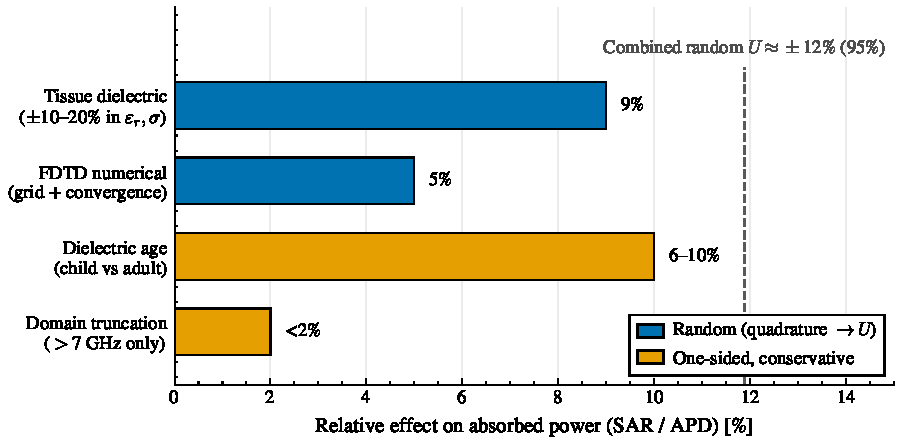
\includegraphics[width=\textwidth]{figures/r32_uncertainty_budget.pdf}
    \caption{Uncertainty budget for the absorbed-power metrics. The tissue-dielectric spread dominates. The \gls{FDTD} numerical error is secondary. These two random terms combine in quadrature to an expanded uncertainty of about~$\pm 12\%$ at a 95\% coverage probability (dashed line). The dielectric-age and domain-truncation effects (orange) act in one direction, conservatively.}
    \label{fig:uncertainty}
\end{figure}

\section{Additional Results and Tables}

This section contains extended numerical tables for directional variation across all four phantoms. These values represent results averaged over the nine FR1 frequencies for each of the 12 incident directions/polarizations.

% Table S3: Duke
\begin{table}[!h]
\centering
\caption{Directional Variation in SAR Metrics (Duke, frequency-averaged values).}
\label{table:direction_var_duke}
\begin{tabular}{@{}lccc@{}}
\toprule
\textbf{Metric} & \textbf{Max} & \textbf{Min} & \textbf{Max/Min} \\
 & \textbf{(mW/kg)} & \textbf{(mW/kg)} & \\
\midrule
Eyes SAR & 28.1 & 1.0 & 28$\times$ \\
Genitals SAR & 15.2 & 0.2 & 67$\times$ \\
Brain SAR & 5.3 & 0.9 & 6$\times$ \\
Skin SAR & 36.0 & 6.0 & 6$\times$ \\
Whole-body SAR & 5.6 & 2.5 & 2$\times$ \\
\bottomrule
\end{tabular}
\end{table}

% Table S4: Ella
\begin{table}[!h]
\centering
\caption{Directional Variation in SAR Metrics (Ella, frequency-averaged values).}
\label{table:direction_var_ella}
\begin{tabular}{@{}lccc@{}}
\toprule
\textbf{Metric} & \textbf{Max} & \textbf{Min} & \textbf{Max/Min} \\
 & \textbf{(mW/kg)} & \textbf{(mW/kg)} & \\
\midrule
Eyes SAR & 32.6 & 0.9 & 36$\times$ \\
Genitals SAR & 2.1 & 0.2 & 9$\times$ \\
Brain SAR & 5.2 & 0.9 & 6$\times$ \\
Skin SAR & 42.9 & 6.7 & 6$\times$ \\
Whole-body SAR & 6.4 & 2.9 & 2$\times$ \\
\bottomrule
\end{tabular}
\end{table}

% Table S5: Eartha
\begin{table}[!h]
\centering
\caption{Directional Variation in SAR Metrics (Eartha, frequency-averaged values).}
\label{table:direction_var_eartha}
\begin{tabular}{@{}lccc@{}}
\toprule
\textbf{Metric} & \textbf{Max} & \textbf{Min} & \textbf{Max/Min} \\
 & \textbf{(mW/kg)} & \textbf{(mW/kg)} & \\
\midrule
Eyes SAR & 41.2 & 1.6 & 27$\times$ \\
Genitals SAR & 4.2 & 0.4 & 10$\times$ \\
Brain SAR & 6.1 & 1.2 & 5$\times$ \\
Skin SAR & 41.8 & 7.8 & 5$\times$ \\
Whole-body SAR & 8.9 & 4.2 & 2$\times$ \\
\bottomrule
\end{tabular}
\end{table}

% Table S6: Thelonious
\begin{table}[!h]
\centering
\caption{Directional Variation in SAR Metrics (Thelonious, frequency-averaged values).}
\label{table:direction_var_thelonious}
\begin{tabular}{@{}lccc@{}}
\toprule
\textbf{Metric} & \textbf{Max} & \textbf{Min} & \textbf{Max/Min} \\
 & \textbf{(mW/kg)} & \textbf{(mW/kg)} & \\
\midrule
Eyes SAR & 28.9 & 1.4 & 20$\times$ \\
Genitals SAR & 30.5 & 0.7 & 46$\times$ \\
Brain SAR & 6.5 & 1.8 & 4$\times$ \\
Skin SAR & 41.3 & 9.2 & 4$\times$ \\
Whole-body SAR & 10.3 & 5.3 & 2$\times$ \\
\bottomrule
\end{tabular}
\end{table}

Figure~\ref{fig:fr1_body_locations} shows where the SAR peak falls within the body for the worst-case focus candidate at each frequency.
At 700~MHz, Duke and Eartha peak in the lower leg, so the 4~W/kg limb basic restriction applies rather than the 2~W/kg head/torso limit.
Ella and Thelonious peak in the torso at both frequencies.
At 3500~MHz, all four phantoms peak in the torso, chest, or neck (54--90\% of body height).

\begin{figure}[!h]
    \centering
    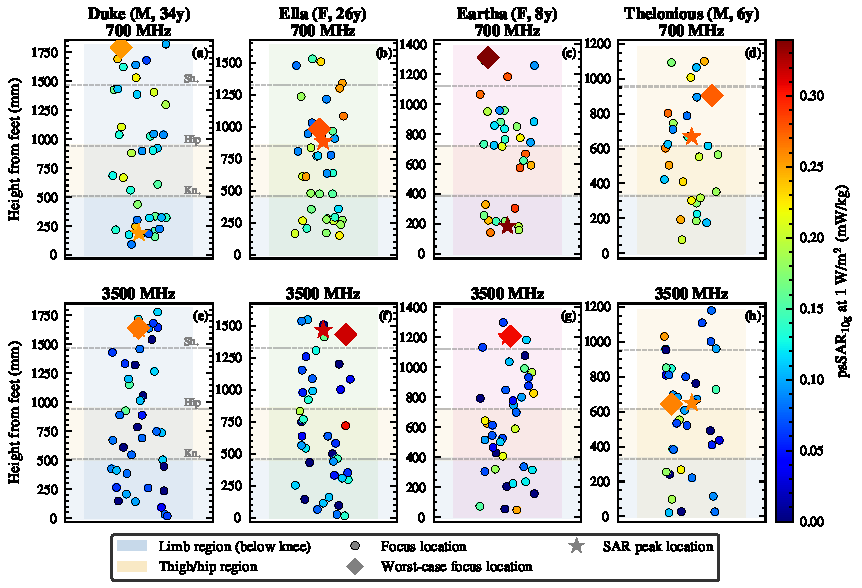
\includegraphics[width=\textwidth]{body_location_figure}
    \caption{Body-height distribution of auto-induced psSAR$_{10\mathrm{g}}$ for FR1 exposure. Circles mark candidate focus locations and a diamond marks the worst-case (highest-SAR) candidate for that phantom and frequency. All symbols are coloured by the resulting psSAR$_{10\mathrm{g}}$ at 1\,W/m$^2$. The star marks where the peak SAR falls within the body for the worst-case candidate. Dashed lines mark approximate anatomical landmarks: Sh.~= shoulder ($\approx$81\%), Hip~= hip ($\approx$52\%), Kn.~= knee ($\approx$28\% of body height from feet). Shaded regions indicate the limb region (blue, below knee) and the thigh/hip region (amber), subject to different ICNIRP basic restriction limits. At 700~MHz, Duke~(a) and Eartha~(c) peak in the lower leg where the limb limit applies. Ella~(b) and Thelonious~(d) peak in the torso. At 3500~MHz all four phantoms peak in the torso, chest, or neck~(e--h).}
    \label{fig:fr1_body_locations}
\end{figure}

\begin{thebibliography}{99}

\bibitem[Bakker \emph{et al}(2010)]{bakker2010children}
Bakker J F, Paulides M M, Christ A, Kuster N and van Rhoon G C 2010 Assessment of induced SAR in children exposed to electromagnetic plane waves between 10~MHz and 5.6~GHz \emph{Phys. Med. Biol.} \textbf{55} 3115--30

\bibitem[Christ \emph{et al}(2010)]{christ2010age}
Christ A, Gosselin M-C, Christopoulou M, K{\"u}hn S and Kuster N 2010 Age-dependent tissue-specific exposure of cell phone users \emph{Phys. Med. Biol.} \textbf{55} 1767--83

\bibitem[Gabriel \emph{et al}(1996)]{gabriel1996dielectric}
Gabriel S, Lau R W and Gabriel C 1996 The dielectric properties of biological tissues: III. Parametric models for the dielectric spectrum of tissues \emph{Phys. Med. Biol.} \textbf{41} 2271--93

\bibitem[Gabriel(2005)]{gabriel2005age}
Gabriel C 2005 Dielectric properties of biological tissue: variation with age \emph{Bioelectromagnetics} \textbf{26} S12--8

\bibitem[Gosselin \emph{et al}(2014)]{gosselin2014development}
Gosselin M-C, Neufeld E, Moser H, Huber E, Farcito S, Gerber L, Jedensj{\"o} M, Hilber I, Di~Gennaro F, Lloyd B, Cherubini E, Szczerba D, Kainz W and Kuster N 2014 Development of a new generation of high-resolution anatomical models for medical device evaluation: The Virtual Population 3.0 \emph{Phys. Med. Biol.} \textbf{59} 5287--303

\bibitem[Hirata \emph{et al}(2021)]{hirata2021review}
Hirata A, Kodera S, Sasaki K, Gomez-Tames J, Laakso I, Wood A, Watanabe S and Foster K R 2021 Human exposure to radiofrequency energy above 6~GHz: review of computational dosimetry studies \emph{Phys. Med. Biol.} \textbf{66} 08TR01

\bibitem[IEC/IEEE(2017)]{iec62704}
IEC/IEEE 2017 62704-1:2017 Determining the peak spatial-average specific absorption rate (SAR) in the human body from wireless communications devices, 30 MHz--6 GHz -- Part 1: General requirements for using the finite-difference time-domain (FDTD) method

\bibitem[IT'IS~Foundation(2024)]{itis_database}
IT'IS Foundation 2024 Tissue Properties Database V5.0 (available at: \url{https://itis.swiss/virtual-population/tissue-properties/database/})

\bibitem[JCGM(2008)]{jcgm2008uncertainty}
JCGM 2008 \emph{Evaluation of Measurement Data---Guide to the Expression of Uncertainty in Measurement} JCGM 100:2008 (Joint Committee for Guides in Metrology) (available at: \url{https://www.bipm.org/documents/20126/2071204/JCGM_100_2008_E.pdf})

\bibitem[Kos \emph{et al}(2011)]{kos2011exposure}
Kos B, Vali\v{c} B, Kotnik T and Gaj\v{s}ek P 2011 Exposure assessment in front of a multi-band base station antenna \emph{Bioelectromagnetics} \textbf{32} 234--42

\bibitem[K{\"u}hn \emph{et al}(2009)]{kuehn2009assessment}
K{\"u}hn S, Jennings W, Christ A and Kuster N 2009 Assessment of induced radio-frequency electromagnetic fields in various anatomical human body models \emph{Phys. Med. Biol.} \textbf{54} 875--90

\bibitem[Peyman \emph{et al}(2009)]{peyman2009dielectric}
Peyman A, Gabriel C, Grant E H, Vermeeren G and Martens L 2009 Variation of the dielectric properties of tissues with age: The effect on the values of SAR in children when exposed to walkie-talkie devices \emph{Phys. Med. Biol.} \textbf{54} 227--41

\bibitem[Taflove and Hagness(2005)]{taflove2005computational}
Taflove A and Hagness S C 2005 \emph{Computational Electrodynamics: The Finite-Difference Time-Domain Method} 3rd edn (Boston: Artech House)

\end{thebibliography}

\end{document}
